% !TEX root = ../SFV15001_MdQM_Fertigungsmesstechnik_Rev01.tex
%
%\frame{\frametitle{Messmethoden}
%\framesubtitle{Unterschied direkte und indirekte Messmethoden}
%\begin{columns}[t] 
%     \begin{column}[T]{6cm} 
%     	\begin{itemize}
%     		\item Direkt:   ohne Hilfsgr\"o{\ss}e die gesuchte Gr\"o{\ss}e
%		
%		\begin{itemize}
%			\item Vergleichend:   Direkter Vergleich mit bekannter Ma{\ss}verk\"orperung
%			\item Ausschlag:   Unmittelbare Anzeige des Gr\"o{\ss}enwertes
%		\end{itemize}
%		\item Indirekt:   Messgr\"o{\ss}e \"uber Hilfsgr\"o{\ss}e  
%		\begin{itemize}
%			\item Hilfsgr\"o{\ss}e: z.B. Widerstand, Volumenstrom
%		\end{itemize}
%     	\end{itemize}
%	\begin{center}
%	\hspace{2cm}\includegraphics[width=0.5\textwidth]{Indirekt}\\
%			\tiny Indirektes Messen eines Innendurchmessers
%			\end{center}
%     \end{column}
%     	\begin{column}[T]{7cm} 
%         	\begin{center}
%            		\includegraphics[width=0.95\textwidth]{DirektIndirekt}\\
%			\tiny Vergleichendes Messen\\
%			\includegraphics[width=0.7\textwidth]{Ausschlag}\\
%			\tiny Ausschlagsmethode
%        		\end{center}
%     \end{column}
% \end{columns}
%}
%
%\frame{\frametitle{Messstrategie}
%\framesubtitle{Neben Messverfahren und Messmethode bestimmt die Antaststrategie ma{\ss}geblich die Messstrategie.}
%     	\begin{itemize}
%     		\item 1-Punkt-Antastung  
%		\begin{itemize}
%			\item Gemeinsamer Bezug (Fl\"ache) zwischen Messmittel und Messgr\"o{\ss}e  
%			\item Beispiel: Tiefenma{\ss}, Durchmesserbestimmung auf Drehtisch  
%		\end{itemize}
%		\item 2-Punkt-Antastung  
%		\begin{itemize}
%			\item Antastung an zwei Fl\"achen, am Schnittpunkt einer Durchsto{\ss}ungsgeraden  
%			\item Beispiel: B\"ugelmessschraube, Messschieber  
%		\end{itemize}
%		\item 3-Punkt-Antastung  
%		\begin{itemize}
%			\item Durchmesserbestimmung: 3 Punkte am Umfang definieren Kreis eindeutig  
%			\item Beispiel: Durchmesserbestimmung mit Prisma
%		\end{itemize}
%     	\end{itemize}
%}
%
%
%\section{Lehrende Pr\"ufung}
%\label{Sec:Lehrend}
%
%\frame{\frametitle{Lehrende Pr\"ufung}
%\framesubtitle{Effiziente Pr\"ufung, ob ein Merkmal in der vorgegebenen Toleranz liegt.}
%\begin{columns}[t] 
%     \begin{column}[T]{6cm} 
%     	\begin{itemize}
%     		\item Schnell
%		\item Nur positiv/negativ Entscheidung
%		\item Ma{\ss}-, Form., Lage- und Sonderlehren:
%		\begin{itemize}
%		\item Sollma{\ss} und -form
%		\item Evtl. einseitiges Grenzma{\ss}
%		\end{itemize}
%		\item Grenzlehren stets zweiseitig oder zweiteilig
%		\begin{itemize}
%		\item Gutseite
%		\item Ausschussseite
%		\end{itemize}
%     	\end{itemize}
%     \end{column}
%     	\begin{column}[T]{5cm} 
%         	\begin{itemize}
%		\item Ma{\ss}lehrung
%		\begin{itemize}
%		\item Pr\"ufstifte, F\"uhlerlehre, Rachenlehre, Lehrdorn
%		\end{itemize}
%		\item Formlehrung
%		\begin{itemize}
%		\item Haarlineal, Profilformlehre
%		\end{itemize}
%		\item Lagelehrung
%		\begin{itemize}
%		\item Winkellehre, Bohrbild
%		\end{itemize}
%		\item Grenzlehrung
%		\begin{itemize}
%		\item Passungslehre
%		\end{itemize}
%		\end{itemize}
%     \end{column}
% \end{columns}
%}
%
%\frame{\frametitle{Taylorscher Grundsatz}
%\framesubtitle{}
%\begin{columns}[t] 
%     \begin{column}[T]{6cm} 
%     	\begin{alertblock}{\color{green!70!black}Gutlehre}
%		Die Gutlehre soll so ausgebildet sein, dass sie die zu pr\"ufende Form in ihrer Gesamtwirkung beurteilt.
%	\end{alertblock}
%	\begin{alertblock}{\color{red!80!black}Ausschusslehre}
%	Die Ausschusslehre soll nur einzelne Bestimmungsst\"ucke der geometrischen Form des Werkst\"ucks pr\"ufen.
%	\end{alertblock}
%     \end{column}
%     	\begin{column}[T]{5cm} 
%         	\begin{center}
%		\only<1>{\includegraphics[width=0.8\textwidth]{BohrungTol}  \begin{center} \tiny
%		Bohrung mit {\color{green!60!black}Kleinstma{\ss}} und {\color{blue!70!black}Toleranz} \end{center}}
%		\only<2>{\includegraphics[width=0.8\textwidth]{Gutlehre} \begin{center} \tiny
%		{\color{green!70!black}Gutlehre} \end{center}}
%		\only<3>{\includegraphics[width=0.8\textwidth]{Ausschusslehre} \begin{center} \tiny
%		{\color{red!80!black}Ausschusslehre} \end{center}}
%        		\end{center}
%     \end{column}
% \end{columns}
%}
%
%
%
%\frame{\frametitle{Ergebnisse der lehrenden Pr\"ufung}
%\framesubtitle{Ergebnisse der lehrenden Pr\"ufung sind mittels diskreter W-Verteilungen zu modellieren.}
%\begin{columns}[t] 
%     \begin{column}[T]{5cm} 
%     	\begin{itemize}
%     		\item Ergebnisse qualitativ, zwei m\"ogliche Ausg\"ange:
%		\begin{itemize}
%		\item Werkst\"uck i.O.
%		\item Werkst\"uck n.i.O.
%		\end{itemize}
%		\item 100\%-Pr\"ufung:
%		\begin{itemize}
%		\item Direkte Entscheidung
%		\end{itemize}
%		\item Stichprobe:  
%		\item Deskriptiv: 
%		\begin{itemize}
%		\item Diagramm
%		\item Quantitativ
%		\end{itemize}
%		\item Induktiv:
%		\begin{itemize}
%		\item Schluss auf Grundgesamtheit
%		\end{itemize}
%     	\end{itemize}
%     \end{column}
%     	\begin{column}[T]{6cm}
%		%\scriptsize 
%         	\textbf{Beispiel:}\\
%		Von einem Produkt mit $p^{\star} = 0{,}01$ Ausschussquote wird eine Stichprobe mit Gr\"o{\ss}e $n = 50$ untersucht. Es werden 
%		\begin{enumerate}
%		\item 1 defektes Teil
%		\item 3 defekte Teile 
%		\end{enumerate}
%		gefunden. Die Binomial-Verteilung
%		\begin{equation*}
%			p(k) = \binom{n}{k} \left(p^{\star}\right)^{k}\left(1 - p^{\star}\right)^{n-k}
%		\end{equation*}
%		ergibt Werte von
%		 $p(1) = 0{,}3056$ und $p(3) = 0{,}0122$.
%     \end{column}
% \end{columns}
%}
%
%\frame{\frametitle{Nomenklatur Hypothesentests und Pr\"ufpl\"ane \cite{kahle13}}
%\framesubtitle{}
%\begin{itemize}
%\item $c:$ Annahmezahl, $c \in \mathbb{N}$
%\item $n$: Stichprobenumfang, $n > c$, $n\geq1$, $n \in \mathbb{N}$
%\item $N$: Anzahl Teile im Los, $n < N$, $N \in \mathbb{N}$
%\item $M$: Ausschussteile im gesamten Los, $M \in \mathbb{N}$
%\item $p^{\star}$: Obere Schranke Ausschussanteil
%\item $p = \frac{M}{N}$: Anteil Ausschussteile im Los
%\item $X$: Anzahl Ausschussteile in Stichprobe, $X \in \mathbb{N}$
%\item Quality Levels:
%	\begin{itemize}
%		\item AQL: Acceptable Quality Level
%		\item IQL: Indifferent Quality Level
%		\item RQL: Rejectable Quality Level
%	\end{itemize}
%\item Risiken:
%\begin{itemize}
%		\item $\alpha$: Herstellerrisiko: Fehlerhafte Ablehnung einer konformen Charge 
%		\item $\beta$: Abnehmerrisiko: Fehlerhafte Annahme einer nicht konformen Charge
%		\end{itemize}
%\end{itemize}
%}
%
%\frame{\frametitle{Hypergeometrische Verteilung}
%\framesubtitle{}
%\begin{itemize}
%\item Dichotome (d.h. mit genau zwei Eigenschaften ausgestattete) Grundgesamtheit
%\begin{itemize}
%	\item z.B. Urne mit Kugeln in zwei Farben
%\end{itemize}
%\item Ziehen ohne Zur\"ucklegen
%\begin{itemize}
%	\item Wahrscheinlichkeit, Kugel einer Farbe zu ziehen ist nicht konstant
%\end{itemize}
%\item F\"ur nat\"urliche Zahlen 
%	\begin{itemize}
%		\item $N$: Gr\"o{\ss}e der Grundgesamtheit
%		\item $M \leq N$ Anzahl Elemente mit Eigenschaft $A$
%		\item $n \leq N$ Gr\"o{\ss}e der Stichprobe und 
%		\item $k\leq n$ Anzahl der Elemente mit Eigenschaft $A$ in der Stichprobe
%	\end{itemize}
%\begin{equation*}
%p(k) = \frac{\binom{M}{k}\binom{N-M}{n-k}}{\binom{N}{n}}
%\end{equation*}
%\item Hoher Rechenaufwand, daher h\"aufig Ann\"aherung durch Binomialverteilung f\"ur $n \ll N$
%\end{itemize}
%}
%
%
%\frame{\frametitle{Hypothesentest}
%\framesubtitle{Um \"uber Ablehnung oder Annahme einer Charge aufgrund einer Stichprobe zu entscheiden, werden Hypothesentests eingesetzt.}
%\begin{columns}[t] 
%     \begin{column}[T]{6cm}
%\begin{itemize}
%\item Nullhypothese $H_{0}$: 
%	\begin{itemize}
%		\item i.d.R. Hypothese, dass das Los konform ist, d.h.\\
%		$H_{0}:\, p \leq p^{\star}$
%		
%		\item f\"ur sicherheitskritische Teile auch Gegenteil
%	\end{itemize}
%\item Alternativhypothese $H_{1}$:
%	\begin{itemize}
%		\item H\"aufig Gegenhypothese zu $H_{0}$, d.h. \\
%		$H_{1}:\, p > p^{\star}$
%	\end{itemize}
%\item Festlegung Signifikanzniveau $\alpha$, typisch 5\% oder 10\%
%\end{itemize}
%\end{column}
%     	\begin{column}[T]{6cm} 
%	\scriptsize
%         	\textbf{Beispiel:}\\ F\"ur Daten wie oben gilt:
%		\begin{itemize}
%		\item $H_{0}$: Charge weist $\leq 1\%$ Ausschuss auf
%		\item $H_{1}$: $H_{0}$ negiert 
%		\item $\alpha = 5\%$
%		\end{itemize}
%		Die kumulierten Wahrscheinlichkeiten laut Binomialverteilung sind:\\ \vspace{0.1cm}
%		\begin{tabular}{|c|c|c|c|c|}
%		\hline
%		$k$ & 0 & 1 & 2& 3 \\ \hline
%		$p(k)$ & 0{,}605 & 0{,}910 & 0,986 & 0{,}988 \\\hline
%		\end{tabular} \\ \vspace{0.1cm}
%		Wegen $p(2) > 0{,}95 = 1-\alpha$ sollen nur Stichproben mit 0 oder 1 defekten Teilen vom Abnehmer angenommen werden, bei 2 oder mehr defekten Teilen wird die Charge abnehmerseitig verworfen.
%     \end{column}
% \end{columns}
%}
%\frame{\frametitle{Pr\"ufpl\"ane und ihre Operationcharakteristik }
%\framesubtitle{Die Operationscharakteristik (OC) stellt die Wahrscheinlichkeit dar, ein Los auf Grundlage einer Pr\"ufstrategie anzunehmen \cite[S. 274ff.]{kahle13}.}
%\begin{columns}[t] 
%     \begin{column}[T]{6.5cm} 
%     	\begin{itemize}
%     		\item OC-Funktion:
%		\begin{equation*}
%		\begin{split}
%			L\left(p, N, N, c \right) = \mathbb{P}\left\{X \leq c \right\} =\\
%			\sum_{i=0}^{c} p_{i}\left(N, M, n\right)
%		\end{split}
%		\end{equation*}
%		\begin{itemize}
%		\item $p_{i}$ mittels Hypergeometrischer Verteilung
%		\item Binomialverteilung als N\"aherung f\"ur $n\ll N$
%		\end{itemize}
%		\item Eigenschaften von $L$:
%		\begin{itemize}
%		\item $L\left(0, N, n, c \right) = 1$
%		\item $L\left(1, N, n, c \right) = 0$
%		\item $L\left(\cdot, N, n, c \right)$ monoton fallend
%		\end{itemize}
%	     	\end{itemize}
%     \end{column}
%     	\begin{column}[T]{6cm} 
%            		% GNUPLOT: LaTeX picture with Postscript
\begingroup
  \makeatletter
  \providecommand\color[2][]{%
    \GenericError{(gnuplot) \space\space\space\@spaces}{%
      Package color not loaded in conjunction with
      terminal option `colourtext'%
    }{See the gnuplot documentation for explanation.%
    }{Either use 'blacktext' in gnuplot or load the package
      color.sty in LaTeX.}%
    \renewcommand\color[2][]{}%
  }%
  \providecommand\includegraphics[2][]{%
    \GenericError{(gnuplot) \space\space\space\@spaces}{%
      Package graphicx or graphics not loaded%
    }{See the gnuplot documentation for explanation.%
    }{The gnuplot epslatex terminal needs graphicx.sty or graphics.sty.}%
    \renewcommand\includegraphics[2][]{}%
  }%
  \providecommand\rotatebox[2]{#2}%
  \@ifundefined{ifGPcolor}{%
    \newif\ifGPcolor
    \GPcolorfalse
  }{}%
  \@ifundefined{ifGPblacktext}{%
    \newif\ifGPblacktext
    \GPblacktexttrue
  }{}%
  % define a \g@addto@macro without @ in the name:
  \let\gplgaddtomacro\g@addto@macro
  % define empty templates for all commands taking text:
  \gdef\gplbacktext{}%
  \gdef\gplfronttext{}%
  \makeatother
  \ifGPblacktext
    % no textcolor at all
    \def\colorrgb#1{}%
    \def\colorgray#1{}%
  \else
    % gray or color?
    \ifGPcolor
      \def\colorrgb#1{\color[rgb]{#1}}%
      \def\colorgray#1{\color[gray]{#1}}%
      \expandafter\def\csname LTw\endcsname{\color{white}}%
      \expandafter\def\csname LTb\endcsname{\color{black}}%
      \expandafter\def\csname LTa\endcsname{\color{black}}%
      \expandafter\def\csname LT0\endcsname{\color[rgb]{1,0,0}}%
      \expandafter\def\csname LT1\endcsname{\color[rgb]{0,1,0}}%
      \expandafter\def\csname LT2\endcsname{\color[rgb]{0,0,1}}%
      \expandafter\def\csname LT3\endcsname{\color[rgb]{1,0,1}}%
      \expandafter\def\csname LT4\endcsname{\color[rgb]{0,1,1}}%
      \expandafter\def\csname LT5\endcsname{\color[rgb]{1,1,0}}%
      \expandafter\def\csname LT6\endcsname{\color[rgb]{0,0,0}}%
      \expandafter\def\csname LT7\endcsname{\color[rgb]{1,0.3,0}}%
      \expandafter\def\csname LT8\endcsname{\color[rgb]{0.5,0.5,0.5}}%
    \else
      % gray
      \def\colorrgb#1{\color{black}}%
      \def\colorgray#1{\color[gray]{#1}}%
      \expandafter\def\csname LTw\endcsname{\color{white}}%
      \expandafter\def\csname LTb\endcsname{\color{black}}%
      \expandafter\def\csname LTa\endcsname{\color{black}}%
      \expandafter\def\csname LT0\endcsname{\color{black}}%
      \expandafter\def\csname LT1\endcsname{\color{black}}%
      \expandafter\def\csname LT2\endcsname{\color{black}}%
      \expandafter\def\csname LT3\endcsname{\color{black}}%
      \expandafter\def\csname LT4\endcsname{\color{black}}%
      \expandafter\def\csname LT5\endcsname{\color{black}}%
      \expandafter\def\csname LT6\endcsname{\color{black}}%
      \expandafter\def\csname LT7\endcsname{\color{black}}%
      \expandafter\def\csname LT8\endcsname{\color{black}}%
    \fi
  \fi
  \setlength{\unitlength}{0.0500bp}%
  \begin{picture}(3400.00,4000.00)%
    \gplgaddtomacro\gplbacktext{%
      \colorrgb{0.00,0.00,0.00}%
      \put(540,400){\makebox(0,0)[r]{\strut{}0}}%
      \colorrgb{0.00,0.00,0.00}%
      \put(540,952){\makebox(0,0)[r]{\strut{}0.2}}%
      \colorrgb{0.00,0.00,0.00}%
      \put(540,1504){\makebox(0,0)[r]{\strut{}0.4}}%
      \colorrgb{0.00,0.00,0.00}%
      \put(540,2055){\makebox(0,0)[r]{\strut{}0.6}}%
      \colorrgb{0.00,0.00,0.00}%
      \put(540,2607){\makebox(0,0)[r]{\strut{}0.8}}%
      \colorrgb{0.00,0.00,0.00}%
      \put(540,3159){\makebox(0,0)[r]{\strut{}1}}%
      \colorrgb{0.00,0.00,0.00}%
      \put(660,200){\makebox(0,0){\strut{}0}}%
      \colorrgb{0.00,0.00,0.00}%
      \put(1136,200){\makebox(0,0){\strut{}0.2}}%
      \colorrgb{0.00,0.00,0.00}%
      \put(1612,200){\makebox(0,0){\strut{}0.4}}%
      \colorrgb{0.00,0.00,0.00}%
      \put(2087,200){\makebox(0,0){\strut{}0.6}}%
      \colorrgb{0.00,0.00,0.00}%
      \put(2563,200){\makebox(0,0){\strut{}0.8}}%
      \colorrgb{0.00,0.00,0.00}%
      \put(3039,200){\makebox(0,0){\strut{}1}}%
    }%
    \gplgaddtomacro\gplfronttext{%
      \colorrgb{0.00,0.00,0.00}%
      \put(3021,3837){\makebox(0,0)[r]{\strut{}$p_i(N, M, n)$}}%
      \colorrgb{0.00,0.00,0.00}%
      \put(3021,3637){\makebox(0,0)[r]{\strut{}$L(p, M, N, c)$}}%
    }%
    \gplbacktext
    \put(0,0){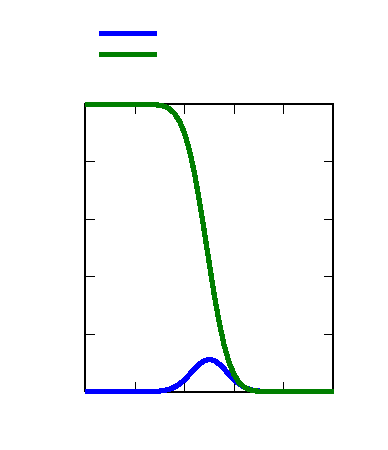
\includegraphics{OC-Funktion}}%
    \gplfronttext
  \end{picture}%
\endgroup

%     \end{column}
% \end{columns}
%}
%\frame{\frametitle{Operationscharakteristik}
%\framesubtitle{}
%\begin{center}
%% GNUPLOT: LaTeX picture with Postscript
\begingroup
  \makeatletter
  \providecommand\color[2][]{%
    \GenericError{(gnuplot) \space\space\space\@spaces}{%
      Package color not loaded in conjunction with
      terminal option `colourtext'%
    }{See the gnuplot documentation for explanation.%
    }{Either use 'blacktext' in gnuplot or load the package
      color.sty in LaTeX.}%
    \renewcommand\color[2][]{}%
  }%
  \providecommand\includegraphics[2][]{%
    \GenericError{(gnuplot) \space\space\space\@spaces}{%
      Package graphicx or graphics not loaded%
    }{See the gnuplot documentation for explanation.%
    }{The gnuplot epslatex terminal needs graphicx.sty or graphics.sty.}%
    \renewcommand\includegraphics[2][]{}%
  }%
  \providecommand\rotatebox[2]{#2}%
  \@ifundefined{ifGPcolor}{%
    \newif\ifGPcolor
    \GPcolorfalse
  }{}%
  \@ifundefined{ifGPblacktext}{%
    \newif\ifGPblacktext
    \GPblacktexttrue
  }{}%
  % define a \g@addto@macro without @ in the name:
  \let\gplgaddtomacro\g@addto@macro
  % define empty templates for all commands taking text:
  \gdef\gplbacktext{}%
  \gdef\gplfronttext{}%
  \makeatother
  \ifGPblacktext
    % no textcolor at all
    \def\colorrgb#1{}%
    \def\colorgray#1{}%
  \else
    % gray or color?
    \ifGPcolor
      \def\colorrgb#1{\color[rgb]{#1}}%
      \def\colorgray#1{\color[gray]{#1}}%
      \expandafter\def\csname LTw\endcsname{\color{white}}%
      \expandafter\def\csname LTb\endcsname{\color{black}}%
      \expandafter\def\csname LTa\endcsname{\color{black}}%
      \expandafter\def\csname LT0\endcsname{\color[rgb]{1,0,0}}%
      \expandafter\def\csname LT1\endcsname{\color[rgb]{0,1,0}}%
      \expandafter\def\csname LT2\endcsname{\color[rgb]{0,0,1}}%
      \expandafter\def\csname LT3\endcsname{\color[rgb]{1,0,1}}%
      \expandafter\def\csname LT4\endcsname{\color[rgb]{0,1,1}}%
      \expandafter\def\csname LT5\endcsname{\color[rgb]{1,1,0}}%
      \expandafter\def\csname LT6\endcsname{\color[rgb]{0,0,0}}%
      \expandafter\def\csname LT7\endcsname{\color[rgb]{1,0.3,0}}%
      \expandafter\def\csname LT8\endcsname{\color[rgb]{0.5,0.5,0.5}}%
    \else
      % gray
      \def\colorrgb#1{\color{black}}%
      \def\colorgray#1{\color[gray]{#1}}%
      \expandafter\def\csname LTw\endcsname{\color{white}}%
      \expandafter\def\csname LTb\endcsname{\color{black}}%
      \expandafter\def\csname LTa\endcsname{\color{black}}%
      \expandafter\def\csname LT0\endcsname{\color{black}}%
      \expandafter\def\csname LT1\endcsname{\color{black}}%
      \expandafter\def\csname LT2\endcsname{\color{black}}%
      \expandafter\def\csname LT3\endcsname{\color{black}}%
      \expandafter\def\csname LT4\endcsname{\color{black}}%
      \expandafter\def\csname LT5\endcsname{\color{black}}%
      \expandafter\def\csname LT6\endcsname{\color{black}}%
      \expandafter\def\csname LT7\endcsname{\color{black}}%
      \expandafter\def\csname LT8\endcsname{\color{black}}%
    \fi
  \fi
  \setlength{\unitlength}{0.0500bp}%
  \begin{picture}(7000.00,3500.00)%
    \gplgaddtomacro\gplbacktext{%
    \put(0,0){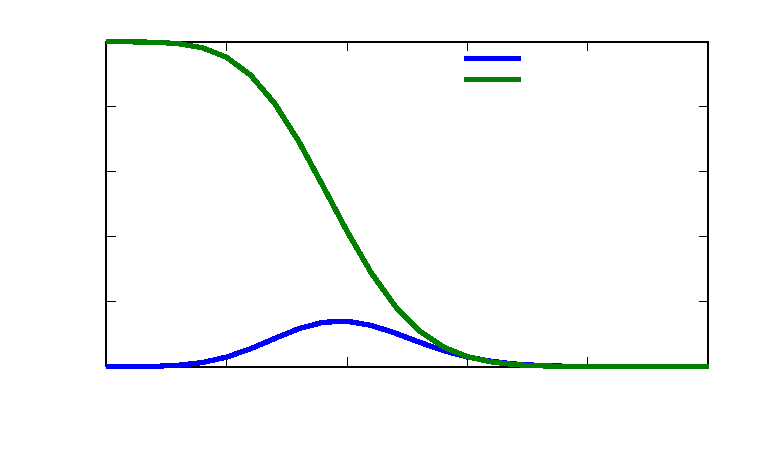
\includegraphics{OC-Funktion2}}
    \thicklines
      \colorrgb{0.00,0.00,0.00}%
      \put(740,640){\makebox(0,0)[r]{\strut{}0}}%
      \colorrgb{0.00,0.00,0.00}%
      \put(740,1264){\makebox(0,0)[r]{\strut{}0.2}}%
      \colorrgb{0.00,0.00,0.00}%
      \put(740,1888){\makebox(0,0)[r]{\strut{}0.4}}%
      \colorrgb{0.00,0.00,0.00}%
      \put(740,2511){\makebox(0,0)[r]{\strut{}0.6}}%
      \colorrgb{0.00,0.00,0.00}%
      \put(740,3135){\makebox(0,0)[r]{\strut{}0.8}}%
      \colorrgb{0.00,0.00,0.00}%
      %%%%%%%%%%
      
      
      \put(860,3759){\makebox(0,0)[r]{\strut{}1}}%
      \colorrgb{0.00,0.00,0.00}%
      \put(860,440){\makebox(0,0){\strut{}0}}%
      \colorrgb{0.00,0.00,0.00}%
      \put(2016,440){\makebox(0,0){\strut{}0.1}}%
      \colorrgb{0.00,0.00,0.00}%
      \put(3172,440){\makebox(0,0){\strut{}0.2}}%
      \colorrgb{0.00,0.00,0.00}%
      \put(4327,440){\makebox(0,0){\strut{}0.3}}%
      \colorrgb{0.00,0.00,0.00}%
      \put(5483,440){\makebox(0,0){\strut{}0.4}}%
      \colorrgb{0.00,0.00,0.00}%
      \put(6639,440){\makebox(0,0){\strut{}0.5}}%
      \colorrgb{0.00,0.00,0.00}%
      \put(160,2199){\rotatebox{90}{\makebox(0,0){\strut{}$L, p_i$}}}%
      \colorrgb{0.00,0.00,0.00}%
      \put(6000,440){\makebox(0,0){\strut{}$p$}}%
    }%
    \gplgaddtomacro\gplfronttext{%
      \colorrgb{0.00,0.00,0.00}%
      \put(6519,3596){\makebox(0,0)[r]{\strut{}$p_i(N, M, n)$}}%
      \colorrgb{0.00,0.00,0.00}%
      \put(6519,3396){\makebox(0,0)[r]{\strut{}$L(p, M, N, c)$}}%
    }%
    \gplbacktext
    %\put(0,0){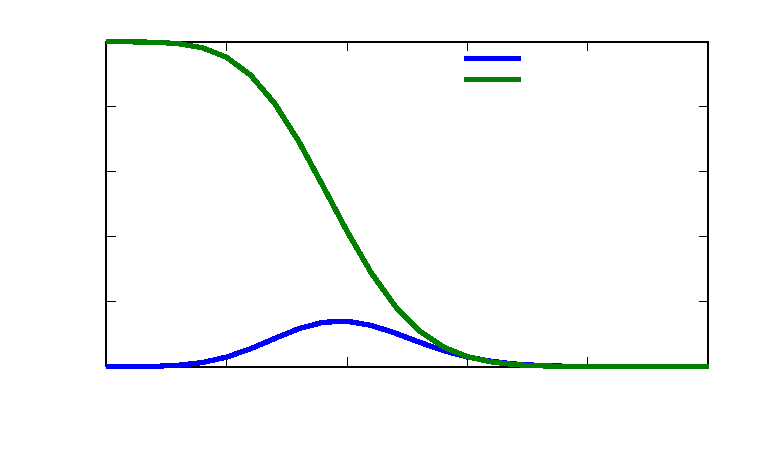
\includegraphics{OC-Funktion2}}%
    \gplfronttext \pause
    \put(2030,3600){\color{red!80!black}
      \put(0,0){\line(-1,0){1180}}
      \put(0,0){\line(0,-1){2960}}
      \put(0,0){\circle*{80}}
      \put(50,0){\makebox(0,0)[l]{\strut{}Produzentenpunkt}}
      \put(-1220,0){\makebox(0,0)[r]{\strut{}$1-\alpha$}}
      \put(0,-3400 ){\makebox(0,0)[c]{\strut{}AQL}}} \pause
      %%%
      \put(3020,2200){\color{red!80!black}
      \put(0,0){\line(-1,0){2160}}
      \put(0,0){\line(0,-1){1550}}
      \put(0,0){\circle*{80}}
      %\put(50,0){\makebox(0,0)[l]{\strut{}Produzentenpunkt}}
      \put(-2200,0){\makebox(0,0)[r]{\strut{}$0{,}5$}}
      \put(0,-2000 ){\makebox(0,0)[c]{\strut{}IQL}}} \pause
      %%%
      \put(3850,1000){\color{red!80!black}
      \put(0,0){\line(-1,0){3000}}
      \put(0,0){\line(0,-1){350}}
      \put(0,0){\circle*{80}}
      \put(50,0){\makebox(0,0)[l]{\strut{}Konsumentenpunkt}}
      \put(-3040,0){\makebox(0,0)[r]{\strut{}$\beta$}}
      \put(0,-800 ){\makebox(0,0)[c]{\strut{}RQL}}}
  \end{picture}%
\endgroup

%\end{center}
%}
%
%\frame{\frametitle{Verhalten einfacher Pr\"ufpl\"ane}
%\framesubtitle{}
%\begin{columns}[t] 
%     \begin{column}[T]{5cm} 
%     	\begin{itemize}
%     		\item Zunehmendes $n$ reduziert IQL-Bereich
%		\item Minimales Risko f\"ur $n = N$
%		\item Mittlerer Pr\"ufaufwand bei abbrechender Kontrolle
%		\begin{equation*}
%		\begin{split}
%		\scriptsize
%		&E = n L\left(p, N, n, c \right) + \\
%		&(c+1) \sum_{l = c+1}^{n}p_{c+1}\left(N, M, l\right)
%		\end{split}
%		\end{equation*}
%
%     	\end{itemize}
%     \end{column}
%     	\begin{column}[T]{7cm} 
%         	\begin{center}
%            		% GNUPLOT: LaTeX picture with Postscript
\begingroup
  \makeatletter
  \providecommand\color[2][]{%
    \GenericError{(gnuplot) \space\space\space\@spaces}{%
      Package color not loaded in conjunction with
      terminal option `colourtext'%
    }{See the gnuplot documentation for explanation.%
    }{Either use 'blacktext' in gnuplot or load the package
      color.sty in LaTeX.}%
    \renewcommand\color[2][]{}%
  }%
  \providecommand\includegraphics[2][]{%
    \GenericError{(gnuplot) \space\space\space\@spaces}{%
      Package graphicx or graphics not loaded%
    }{See the gnuplot documentation for explanation.%
    }{The gnuplot epslatex terminal needs graphicx.sty or graphics.sty.}%
    \renewcommand\includegraphics[2][]{}%
  }%
  \providecommand\rotatebox[2]{#2}%
  \@ifundefined{ifGPcolor}{%
    \newif\ifGPcolor
    \GPcolorfalse
  }{}%
  \@ifundefined{ifGPblacktext}{%
    \newif\ifGPblacktext
    \GPblacktexttrue
  }{}%
  % define a \g@addto@macro without @ in the name:
  \let\gplgaddtomacro\g@addto@macro
  % define empty templates for all commands taking text:
  \gdef\gplbacktext{}%
  \gdef\gplfronttext{}%
  \makeatother
  \ifGPblacktext
    % no textcolor at all
    \def\colorrgb#1{}%
    \def\colorgray#1{}%
  \else
    % gray or color?
    \ifGPcolor
      \def\colorrgb#1{\color[rgb]{#1}}%
      \def\colorgray#1{\color[gray]{#1}}%
      \expandafter\def\csname LTw\endcsname{\color{white}}%
      \expandafter\def\csname LTb\endcsname{\color{black}}%
      \expandafter\def\csname LTa\endcsname{\color{black}}%
      \expandafter\def\csname LT0\endcsname{\color[rgb]{1,0,0}}%
      \expandafter\def\csname LT1\endcsname{\color[rgb]{0,1,0}}%
      \expandafter\def\csname LT2\endcsname{\color[rgb]{0,0,1}}%
      \expandafter\def\csname LT3\endcsname{\color[rgb]{1,0,1}}%
      \expandafter\def\csname LT4\endcsname{\color[rgb]{0,1,1}}%
      \expandafter\def\csname LT5\endcsname{\color[rgb]{1,1,0}}%
      \expandafter\def\csname LT6\endcsname{\color[rgb]{0,0,0}}%
      \expandafter\def\csname LT7\endcsname{\color[rgb]{1,0.3,0}}%
      \expandafter\def\csname LT8\endcsname{\color[rgb]{0.5,0.5,0.5}}%
    \else
      % gray
      \def\colorrgb#1{\color{black}}%
      \def\colorgray#1{\color[gray]{#1}}%
      \expandafter\def\csname LTw\endcsname{\color{white}}%
      \expandafter\def\csname LTb\endcsname{\color{black}}%
      \expandafter\def\csname LTa\endcsname{\color{black}}%
      \expandafter\def\csname LT0\endcsname{\color{black}}%
      \expandafter\def\csname LT1\endcsname{\color{black}}%
      \expandafter\def\csname LT2\endcsname{\color{black}}%
      \expandafter\def\csname LT3\endcsname{\color{black}}%
      \expandafter\def\csname LT4\endcsname{\color{black}}%
      \expandafter\def\csname LT5\endcsname{\color{black}}%
      \expandafter\def\csname LT6\endcsname{\color{black}}%
      \expandafter\def\csname LT7\endcsname{\color{black}}%
      \expandafter\def\csname LT8\endcsname{\color{black}}%
    \fi
  \fi
  \setlength{\unitlength}{0.0500bp}%
  \begin{picture}(4000.00,3500.00)%
    \gplgaddtomacro\gplbacktext{%
      \colorrgb{0.00,0.00,0.00}%
      \put(540,640){\makebox(0,0)[r]{\strut{}0}}%
      \colorrgb{0.00,0.00,0.00}%
      \put(540,1192){\makebox(0,0)[r]{\strut{}0.2}}%
      \colorrgb{0.00,0.00,0.00}%
      \put(540,1744){\makebox(0,0)[r]{\strut{}0.4}}%
      \colorrgb{0.00,0.00,0.00}%
      \put(540,2295){\makebox(0,0)[r]{\strut{}0.6}}%
      \colorrgb{0.00,0.00,0.00}%
      \put(540,2847){\makebox(0,0)[r]{\strut{}0.8}}%
      \colorrgb{0.00,0.00,0.00}%
      \put(540,3399){\makebox(0,0)[r]{\strut{}1}}%
      \colorrgb{0.00,0.00,0.00}%
      \put(660,440){\makebox(0,0){\strut{}0}}%
      \colorrgb{0.00,0.00,0.00}%
      \put(1157,440){\makebox(0,0){\strut{}0.05}}%
      \colorrgb{0.00,0.00,0.00}%
      \put(1653,440){\makebox(0,0){\strut{}0.1}}%
      \colorrgb{0.00,0.00,0.00}%
      \put(2150,440){\makebox(0,0){\strut{}0.15}}%
      \colorrgb{0.00,0.00,0.00}%
      \put(2646,440){\makebox(0,0){\strut{}0.2}}%
      \colorrgb{0.00,0.00,0.00}%
      \put(3143,440){\makebox(0,0){\strut{}0.25}}%
      \colorrgb{0.00,0.00,0.00}%
      \put(3639,440){\makebox(0,0){\strut{}0.3}}%
      \colorrgb{0.00,0.00,0.00}%
      \put(2149,140){\makebox(0,0){\strut{}$p$}}%
      \csname LTb\endcsname%
      \put(2149,3699){\makebox(0,0){\strut{}OC für $N = 1000$, $p^{\star} = 0{,}1$}}%
    }%
    \gplgaddtomacro\gplfronttext{%
      \colorrgb{0.00,0.00,0.00}%
      \put(3519,3236){\makebox(0,0)[r]{\strut{}$n= 50$}}%
      \colorrgb{0.00,0.00,0.00}%
      \put(3519,3036){\makebox(0,0)[r]{\strut{}$n= 100$}}%
      \colorrgb{0.00,0.00,0.00}%
      \put(3519,2836){\makebox(0,0)[r]{\strut{}$n= 500$}}%
      \colorrgb{0.00,0.00,0.00}%
      \put(3519,2636){\makebox(0,0)[r]{\strut{}$n= 1000$}}%
    }%
    \gplbacktext
    \put(0,0){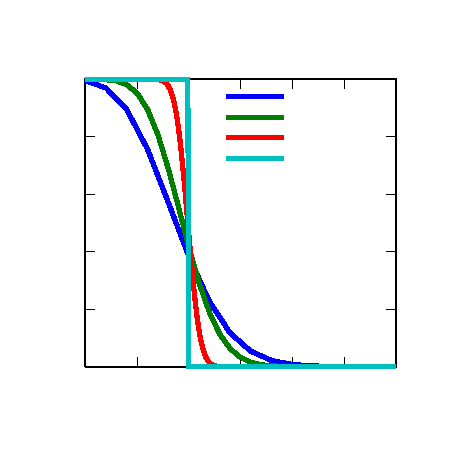
\includegraphics{OC-Funktion3}}%
    \gplfronttext
  \end{picture}%
\endgroup

%        		\end{center}
%     \end{column}
% \end{columns}
%}

%\frame{\frametitle{Algorithmus zur Erstellung einfacher Pr\"ufpl\"ane}
%\framesubtitle{}
%\begin{columns}[t] 
%     \begin{column}[T]{5cm} 
%     	\begin{itemize}
%     		\item 
%     	\end{itemize}
%     \end{column}
%     	\begin{column}[T]{7cm} 
%         	\begin{picture}(200, 200)(-100,-200)
%	\thicklines
%	\scriptsize
%            		\put(0,0){\oval(100,16)[8]}
%			\put(0,0){\makebox(0,0)[c]{\strut{}Eingabe $\alpha$, $\beta$, $p_{\alpha}$, $p_{\beta}$, $N$}}
%			\put(0,-8){\vector(0,-1){8}}
%			\put(0,0){\oval(100,16)[8]}
%			\put(0,0){\makebox(0,0)[c]{\strut{}Eingabe $\alpha$, $\beta$, $p_{\alpha}$, $p_{\beta}$, $N$}}
%        		\end{picture}
%     \end{column}
% \end{columns}
%}
